\documentclass[12pt, a4paper, oneside]{ctexart}
\usepackage{amsmath, amsthm, amssymb, bm, color, graphicx, geometry, mathrsfs,extarrows, braket, booktabs, array, xcolor, fontspec, appendix, float, subfigure, wrapfig, enumitem, titlesec}
\usepackage[colorlinks,linkcolor=red,anchorcolor=blue,citecolor=blue,urlcolor=blue,menucolor=black]{hyperref}

%%%% 设置中文字体 %%%%
\setCJKmainfont{方正新书宋_GBK.ttf}[BoldFont = 方正小标宋_GBK, ItalicFont = 方正楷体_GBK, BoldItalicFont = 方正粗楷简体]
%%%% 设置英文字体 %%%%
\setmainfont{Times New Roman}
\setsansfont{Calibri}
\setmonofont{Consolas}

%%%% 设置代码块 %%%%
% 在vscode中使用minted需要先配置python解释器, Ctrl+Shift+P, 输入Python: Select Interpreter选择安装了Pygments的Python版本. 再在setting.json中xelatex和pdflatex的参数中加入 "--shell-escape", 即可
% TeXworks中配置方法参考: https://blog.csdn.net/RobertChenGuangzhi/article/details/108140093
\usepackage{minted}
\renewcommand{\theFancyVerbLine}{
    \sffamily\textcolor[rgb]{0.5,0.5,0.5}{\scriptsize\arabic{FancyVerbLine}}} % 修改代码前序号大小
% 加入不同语言的代码块,数学公式使用方法 $公式$
\newmintinline{cpp}{fontsize=\small, linenos, breaklines, frame=lines}
\newminted{cpp}{fontsize=\small, mathescape=true, baselinestretch=1, linenos, breaklines, frame=lines}
\newmintedfile{cpp}{fontsize=\small, mathescape=true, baselinestretch=1, linenos, breaklines, frame=lines}
\newmintinline{matlab}{fontsize=\small, linenos, breaklines, frame=lines}
\newminted{matlab}{fontsize=\small, baselinestretch=1, mathescape, linenos, breaklines, frame=lines}
\newmintedfile{matlab}{fontsize=\small, baselinestretch=1, linenos, breaklines, frame=lines}
\newmintinline{python}{fontsize=\small, linenos, breaklines, frame=lines, python3}  % 使用\pythoninline{代码}
\newminted{python}{fontsize=\small, baselinestretch=1, linenos, breaklines, frame=lines, python3}  % 使用\begin{pythoncode}代码\end{pythoncode}
\newmintedfile{python}{fontsize=\small, baselinestretch=1, linenos, breaklines, frame=lines, python3}  % 使用\pythonfile{代码地址}

%%%% 设置行间距与页边距 %%%%
\linespread{1.2}
\geometry{left=1.84cm,right=1.84cm,top=2.18cm,bottom=2.18cm}

%%%% 定理类环境的定义 %%%%
\newtheorem{theorem}{定理}[section] % 定理按section编号
\newtheorem{definition}{定义}[section]
\newtheorem{axiom}{公理}
\newtheorem{property}{性质}
\newtheorem{proposition}{命题}
\newtheorem{lemma}{引理}
\newtheorem{corollary}{推论}
\newtheorem{condition}{条件}
\newtheorem{conclusion}{结论}
\newtheorem{assumption}{假设}
\numberwithin{equation}{section}  % 公式按section编号 (公式右端的小括号)
\newtheorem{algorithm}{算法}
\theoremstyle{definition}
\newtheorem{example}{例}[section]

%%%% 自定义环境 %%%%
\newsavebox{\nameinfo}
\newenvironment{myTitle}[1]{
    \begin{center}
    {\zihao{-2}\bf #1\\}
    \zihao{-4}\it
}{\end{center}}  % \begin{myTitle}{标题内容}作者信息\end{myTitle}
\newcounter{problem}  % 问题序号计数器
\newenvironment{problem}[1][]{\stepcounter{problem}\par\noindent\textbf{题目\arabic{problem}. #1}}{\smallskip\par}
\newenvironment{solution}[1][]{\par\noindent\textbf{#1解答. }}{\smallskip\par}  % 可带一个参数表示题号\begin{solution}{题号}
\newenvironment{note}{\par\noindent\textbf{注记. }}{\smallskip\par}
\newenvironment{remark}{\begin{enumerate}[label=\textbf{注\arabic*.}]}{\end{enumerate}}
\BeforeBeginEnvironment{minted}{\vspace{-0.5cm}}  % 缩小minted环境距上文间距
\AfterEndEnvironment{minted}{\vspace{-0.2cm}}  % 缩小minted环境距下文间距

%%%% 自定义段落开头 %%%%
\titleformat{\section}{\Large\bfseries}{第\zhnum{section}章}{1em}{}[]

%%%% 图片相对路径 %%%%
\graphicspath{{figures/}} % 当前目录下的figures文件夹, {../figures/}则是父目录的figures文件夹
\setlength{\abovecaptionskip}{-0.2cm}  % 缩紧图片标题与图片之间的距离
\setlength{\belowcaptionskip}{0pt} 

%%%% 缩小item,enumerate,description两行间间距 %%%%
\setenumerate[1]{itemsep=0pt,partopsep=0pt,parsep=\parskip,topsep=5pt}
\setitemize[1]{itemsep=0pt,partopsep=0pt,parsep=\parskip,topsep=5pt}
\setdescription{itemsep=0pt,partopsep=0pt,parsep=\parskip,topsep=5pt}

%%%% 自定义公式 %%%%
\everymath{\displaystyle} % 默认全部行间公式, 想要变回行内公式使用\textstyle
\DeclareMathOperator*\uplim{\overline{lim}}     % 定义上极限 \uplim_{}
\DeclareMathOperator*\lowlim{\underline{lim}}   % 定义下极限 \lowlim_{}
\DeclareMathOperator*{\argmax}{arg\,max}  % 定义取最大值的参数 \argmax_{}
\DeclareMathOperator*{\argmin}{arg\,min}  % 定义取最小值的参数 \argmin_{}
\let\leq=\leqslant % 简写小于等于\leq (将全部leq变为leqslant)
\let\geq=\geqslant % 简写大于等于\geq (将全部geq变为geqslant)
\DeclareRobustCommand{\rchi}{{\mathpalette\irchi\relax}}
\newcommand{\irchi}[2]{\raisebox{\depth}{$#1\chi$}} % 使用\rchi将\chi居中

%%%% 一些宏定义 %%%%
\def\bd{\boldsymbol}        % 加粗(向量) boldsymbol
\def\disp{\displaystyle}    % 使用行间公式 displaystyle(默认)
\def\tsty{\textstyle}       % 使用行内公式 textstyle
\def\sign{\text{sign}}      % sign function
\def\wtd{\widetilde}        % 宽波浪线 widetilde
\def\R{\mathbb{R}}          % Real number
\def\N{\mathbb{N}}          % Natural number
\def\Z{\mathbb{Z}}          % Integer number
\def\Q{\mathbb{Q}}          % Rational number
\def\C{\mathbb{C}}          % Complex number
\def\K{\mathbb{K}}          % Number Field
\def\P{\mathbb{P}}          % Polynomial
\def\d{\mathrm{d}}          % differential operator
\def\e{\mathrm{e}}          % Euler's number
\def\i{\mathrm{i}}          % imaginary number
\def\re{\mathrm{Re}}        % Real part
\def\im{\mathrm{Im}}        % Imaginary part
\def\res{\mathrm{Res}}      % Residue
\def\ker{\mathrm{Ker}}      % Kernel
\def\vspan{\mathrm{vspan}}  % Span  \span与latex内核代码冲突改为\vspan
\def\L{\mathcal{L}}         % Loss function
\def\O{\mathcal{O}}         % 
\def\wdh{\widehat}          % 宽帽子 widehat
\def\ol{\overline}          % 上横线 overline
\def\ul{\underline}         % 下横线 underline
\def\add{\vspace{1ex}}      % 增加行间距
\def\del{\vspace{-1.5ex}}   % 减少行间距

\begin{document}
\section{NP完全性理论}
\subsection{概念}
\begin{definition}[确定性算法与非确定性算法]
    \begin{itemize}
        \item \textbf{确定性算法}:算法中每个操作结果唯一确定,算法操作结果也是唯一确定.
        \item \textbf{非确定性算法}:算法操作结果不唯一,而是来自可能值集合.
    \end{itemize}
\end{definition}
这里的确定性算法指的就是非随机算法,非确定性算法就是随机算法,可能值集合也就是可行解.

\begin{definition}[判定问题,判定算法]
    答案非0即1的所有问题称为判定问题,求解判定问题的算法称为判定算法.
\end{definition}

往往将可在多项式时间内解决的问题视为“易”解问题,需要指数时间及以上解决的问题称为“难”解问题. 为了详细区分这两种问题,引入了P类问题和NP类问题,
首先要注意,NP问题不是指不能在多项式时间内求解的问题,而是值\textbf{无法确定}是否可在多项式时间内求解的问题,因为可能通过随机算法,
运气好直接碰出答案了,所以需要用算法的确定性对其进行定义.

\begin{definition}[P类问题]
    在多项式时间内,可使用确定性算法求解的判定问题构成的集合.
\end{definition}

\begin{definition}[NP类问题]
    在多项式时间内,可使用非确定性算法求解的判定问题构成的集合.
\end{definition}

在默认使用的均是确定性算法前提下,可以P类问题与NP类问题可以如下表示:
\begin{align*}
    \text{P类问题} =&\ \{\text{判定问题}:\text{可在多项式时间内\textbf{求出}正确解}\}\\
    \text{NP类问题} =&\ \{\text{判定问题}:\text{无法确定是否可在多项式时间内求出正确解}\}\\
    =&\ \{\text{问题}:\text{可在多项式的时间内\textbf{验证}是否得出正确解}\}
\end{align*}
可以从上述NP类问题的第二种定义可以看出,将问题转化为“判定问题”是必要的,使得验证时间为$\O(1)$,仅需关心求解所需的时间复杂度. 
证明一个问题是否是NP问题,只需判断\textbf{是否可以在多项式时间内验证是否为正确解}.

由定义可知,$\text{P}\subset \text{NP}$,但P是否等于NP是世纪难题.

在引入NP完全问题和NP难定义前,先给出这些定义之间的逻辑关系:由于没有定义NP问题就是不能在多项式时间内求解的问题,
所以还是可能存在一种线性算法使其能在多项式时间内给出正确解,只是人们还没有发现
(如果$\text{P} = \text{NP}$则说明全部的NP问题都能多项式时间内解决,而且这种“可能”现在有可能可以通过量子计算机完成). 
对于NP问题$A$,通过“多项式时间变换”,将NP问题$A$变换为更为复杂的NP问题$B$,如果可以多项式时间内求解NP问题$B$,
则可以求解NP问题$A$,人们将比所有NP问题都更难的那部分NP问题称为NP完全问题,并将比所有NP都要难的问题通称为NP难问题.

\begin{definition}[多项式时间变换]
    设$X,Y$分别是定义在实例集$I,J$上的两个判定问题,若存在从$I$到$J$的映射$f:I\to J$使得
    \begin{enumerate}
        \item $f$是在多项式时间内可计算的映射.
        \item $\{f(x):x\in X\} \subset Y$
    \end{enumerate}
    则称问题$X$能\textbf{多项式时间变换}为问题$Y$,记为$X\propto_p Y$.
\end{definition}
\begin{definition}[NP完全问题,NPC]
    设$Y\in \text{NP}$,则$Y$是NP完全的,当且仅当,
    \begin{enumerate}
        \item $Y\in NP$.
        \item $\forall X\in \text{NP}$有$X\propto_p Y$.
    \end{enumerate}
    将全体NP完全问题,记为NP完全类,简写为NPC.
\end{definition}
\begin{definition}[NP难问题,NP-Hard]
    设$Y\in \text{NP}$,则$Y$是NP难的,当且仅当,$\forall X\in \text{NP}$有$X\propto_p Y$.(即满足NP完全问题中的第二条即可)
\end{definition}
P, NP, NPC, NP-Hard问题关系如下图\footnote{By Behnam Esfahbod, CC BY-SA 3.0, https://commons.wikimedia.org/w/index.php?curid=3532181}
所示,纵轴显示了解决问题的难度:
\begin{figure}[htbp]
    \centering
    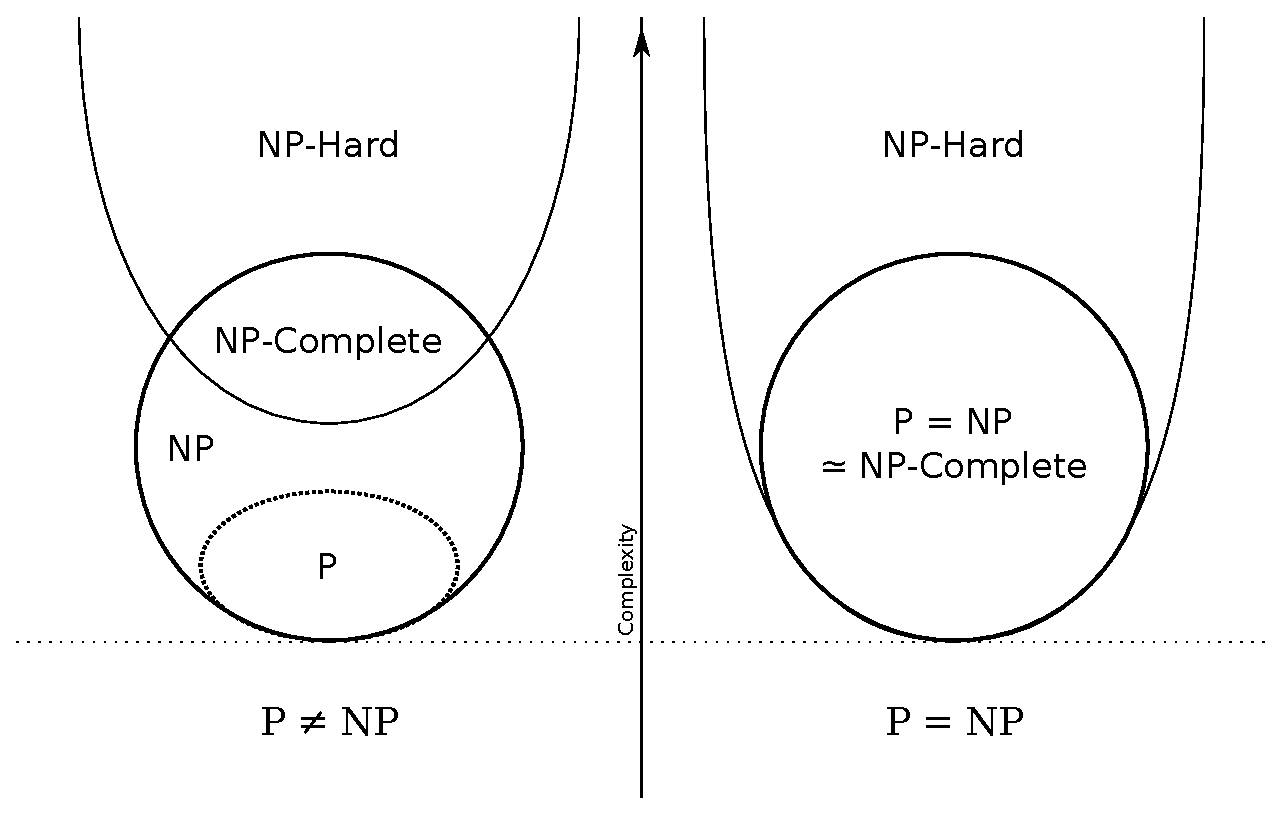
\includegraphics[scale=0.5]{P_np_np-complete_np-hard.eps}
\end{figure}

\subsection{判断一个问题是否是NP完全问题}
首先要记住几个经典的NP完全问题(重要的问题会在文末详细给出):布尔表达式可满足问题(SAT),合取范式的可满足问题(CNF-SAT),三元合取范式可满足问题(3-SAT),
k团问题(CLIQUE),k顶点覆盖问题(VERTEX-COVER),子集和问题(SUBSET-SUM),哈密顿回路问题(HAM-CYCLE),旅行商问题(TSP).

\textbf{Cook定理}说明SAT是NP完全问题,上述相邻的两个问题,前一个问题可通过多项式时间变换转化为后一个问题.

\textbf{证明一个问题$A$是否是NP完全问题}:假设已知问题$B$是NP完全问题,根据定义,只需证$A$是NP问题且$A$是$B$的NP完全问题即可. 

第一步:证明$A$是NP问题,即是否可以在多项式时间内给出\textbf{验证}是否是问题$A$的正确解.

第二步:找一个多项式时间内的映射,将问题$B$映射到问题$A$上即可.

若只需证明$A$是NP难问题,则只需证明第二步.

\textbf{k团问题(CLIQUE)}:给定一个无向图$G=(V,E)$和一个正整数$k$,判定图$G$是否包含一个大小为$k$的团,
即是否存在,$V’\subset V,\ |V’|=k$且$\forall u, w\in V’$有$(u,w)\in E$.

\textbf{k顶点覆盖问题(VERTEX-COVER)}:给定一个无向图$G=(V,E)$和一个正整数$k$,判定是否存在$V’\subset V, |V’|=k$,
使得$\forall (u,v)\in E$有$u\in V’$或$v\in V’$. 若存在这样的$V’$,则称$V’$为图$G$的一个大小为$k$顶点覆盖.

\textbf{子集和问题(SUBSET-SUM)}:给定整数集合$S$和一个整数$t$,判定是否存在$S$的一个子集$S’\subset S$,使得$S’$中整数的和为$t$.

\textbf{哈密顿回路问题(HAM-CYCLE)}:给定无向图$G=(V,E)$,判定其是否含有哈密顿回路,即判定$G$是否存在经过$V$中各顶点恰好一次的回路.

\textbf{旅行商问题(TSP)}:给定一个无向完全图$G=(V,E)$及定义在$V\times V$上的一个费用函数$c$和一个整数$k$,
判定$G$是否存在经过$V$中各顶点恰好一次的回路,使得该回路的费用不超过$k$.
\end{document}
